\clearpage
\section{Parametric model of the wrist motion}

We aim at creating a parametric model of the wrist motion, such that the parameters are interpretable by a human user. The idea is to create an example of a healthy wrist, whose bones follow a standard motion. It can be used to help diagnose unhealthy wrist patterns, by comparison between the healthy model movement and the one observed from an individual. Such a model is based on the hypothesis that continuous movement can be inferred from some poses, which has already been discussed in \cite{foumani_2009_vivo}. 
%We also assume that the motion is linear between poses, the same hypothesis was made in the literature using the PCA-based models. 
The necessity of interpretable parameters comes from the utilization of the model for diagnosis: if the parameters describe the angles of the wrist and thumb in \fe* and \aa*, it is really easy for an individual to take a certain wrist pose and report the parameters into the model for comparison. 

We base our method on a simple multiple regression analysis. First we briefly present the mathematical background of the model, then we describe how our model was constructed and the results obtained. 


\subsection{Multiple regression analysis}

Multiple regression analysis is a supervised learning technique, whose purpose is to determine the relationship between some predictor (independent) variables $\mathbf{x}$ and a dependent variable $\mathbf{y}$. 

\begin{equation}
	\mathbf{y} \approx f(\mathbf{x}, \beta)
	\label{eq:multiple_regression}
\end{equation}

We are only interested in linear regression, that is the dependent variables can be described as a linear combination of the regression parameters $\beta$. It is not necessarily a linear combination of the predictors and non linear functions $\Phi$ of each predictor can be used, such as any degree polynomial function or any kernel-based function \cite{zhuang_2017_statistical}. The major advantage of linear regression is that it can be efficiently solved using least-squares. In linear regression, equation \eqref{eq:multiple_regression} for $p$ predictor variables and $r$ dependent variables can be written as : 

\begin{equation}
	\mathbf{y}_k = \beta_{1,k} \Phi_1(x_{1}) + \beta_{2,k} \Phi_2(x_{2}) + ... + \beta_{p,k} \Phi_p(x_{p})
\end{equation}

$\mathbf{y}_k$ is the $k^{th}$ dependent variable, $k\in \{1,..,r\}$. 
The parameters $\beta_{j,k}$ are computed using the training set, which is such that both observed predictors $\widehat{x}$ and the associated observed $\widehat{y}$ are known. Let $\mathbf{\Phi}$ be the matrix such that $\mathbf{\Phi}_{i,j} = \Phi_j(\widehat{x_{i,j}})$, $\widehat{x_{i,j}}$ is the $i^{th}$ observation of the $j^{th}$ predictor. In matrix notation, 

\begin{equation}
	Y = \mathbf{\Phi} \Beta
\end{equation}

If there are $n$ observations, $p$ predictors and $r$ dependent variables, then $\mathbf{\Phi}$ is $n\times p$, $Y$ is $n\times r$ and $\Beta$ is $p\times r$.
The regression parameters are computed using: 

\begin{equation}
	\Beta = \left( \mathbf{\Phi}^t \mathbf{\Phi}\right)^{-1} \mathbf{\Phi}^t Y
	\label{eq:regression_computation}
\end{equation}

A regularization parameter $\lambda$ can be added to avoid overfitting: 

\begin{equation}
	\Beta = \left( \mathbf{\Phi}^t \mathbf{\Phi} + \lambda I\right)^{-1} \mathbf{\Phi}^t Y
	\label{eq:regression_regularization}
\end{equation}

In the next subsection, we describe how multiple regression analysis is used to model the wrist pose of all bones. 

\subsection{Parametric model}
\label{ssec:parametric_model}

We want to parameterize the pose of a wrist with interpretable parameters, we define 5 of them: 4 parameters characterize the degrees of freedom of the thumb and wrist articulations: the degree of rotation in \textit{\fe* of the wrist}, the degree of rotation in \textit{radial-ulnar deviation of the wrist}, the degrees of rotation in \textit{\fe*} and \textit{\aa* of the thumb}. A last boolean parameter describes whether the pose is \textit{loaded}, that is if the individual puts some force in the pose or not. The parameters describe all degrees of freedom of the joints we aim at modeling. They should therefore be able to capture the whole range of possible poses. Additionally, they are easily measurable, both for a living human being, with a goniometer for instance, and for a computer wrist pose characterized by 3D meshes of the bones, as detailed in \tabref{tab:parameter_regression_computation}. It only requires to know the neutral pose, since the parameters are expressed relatively to it.

In both NIH and \db*s, a pose is described as a list of matrices defining for each bone the rigid transformations from the neutral pose to the current one. We have to estimate the values of the model parameters from the wrist bones movements. The angles of rotation of the \mcu* and \mct* bones are used to characterize respectively the thumb and the wrist angles. A \soc* is defined on the radius, as described in \secref{ssubsec:rough_ali}. A \soc* parallel to the radius one at neutral pose is defined on the \mct*. The \textit{global wrist angles} are calculated as the angles of the \mct* with respect to the radius \cite{patterson_1998_high}, as listed in \tabref{tab:parameter_regression_computation}. For example, rotation about the $Y$ axis describes the angle of \fe*, if the angle is positive, the wrist is in flexion, if negative the wrist is in extension. The rotations values are $0$ when the wrist is in its neutral pose. For the description of the \textit{thumb angle}, the movement of the \mcu* relatively to the \tpm* is used. A joint coordinate system on the TMC joint is computed, its definition is the one described in \secref{sec:4_CoordSys}, our method based on the correspondence property is applied. The thumb angles (\tabref{tab:parameter_regression_computation}) are described as defined in \cite{halilaj_2013_thumb}. Once again, the angles are considered to be $0$ at neutral pose.

\begin{table}
	\centering
	\begin{tabular}{lccc}
		\toprule
		Parameter & Movement of & Relatively to & Rotation axis \\
		\midrule
		Wrist \fe* & \mct* & \rad* & $Y_\text{RAD}$ \\
		Wrist deviation & \mct* & \rad* & $X_\text{RAD}$ \\
		Thumb \fe* & \mcu* & \tpm* & $Z_\text{TPM}$ \\
		Thumb \aa* & \mcu* & \tpm* & $X_\text{MC1}$ \\
		\bottomrule
	\end{tabular}
	\caption[Computation of the statistical movement model parameters]{The parameters values are the angles of rotation of a bone relatively to another one, around particular axis of systems of coordinates defined in \secref{ssec:parametric_model}. }
	\label{tab:parameter_regression_computation}
\end{table}



\subsection{Model application}


We are interested in working both with wrist and thumb movements, therefore we work with the \db*. The poses mostly are about thumb movement: the 10 poses, in addition to the neutral one are: thumb flexion and extension; thumb adduction and abduction; pinch, jar grasp and jar twist with and without load (\tabref{tab:poses_CMC} ). However, we observe a residual movement of the wrist, which is not completely motionless between poses. This residual movement consists mostly in extension and radial-ulnar deviation. It enables to consider that both wrist and thumb movements can be modeled. The presence of residual wrist movement was confirmed using a PCA on the movement data. The NIH database for its part is composed of poses of the wrist movement, but thumb movements are absent. 


%We make the assumption that each subject has a unique way of moving its wrist that depends on its bones shapes. 
It has been proved for example that two types of lunate exist, and the type of the bone influences the kinematics of the neighboring bones \cite{nakamura_2000_motion, galley_2007_influence, bain_2015_effect}. Therefore each subject is considered separately, one model is created for each person. Ideally a future model will be able to consider all subjects together, by considering the bones shapes characterized by a statistical shape model as a parameter of the person. The model should be able to adapt the motion modeled to an individual's anatomy. However we have not yet succeeded in creating such a model.

A bone in pose $P$ is characterized by the translation and rotation undergone from its neutral position and orientation to the pose $P$. It is a vector of size $6$: $v = (r_x, r_y, r_z,\allowbreak t_x, t_y, t_z)$. The rotation is measured with Euler angles. One pose is represented by the concatenation of all bone vectors for this pose. It is a vector of size $6B$, with $B=14$ the number of wrist bones (8 carpals, 5 metacarpals and the radius). The motion space defined by the poses of the data is calculated for one individual at a time, since we expect the motion to be dependent on the person. Using the same notations as in \eqref{eq:regression_computation}, $n=11$ is the number of poses for one individual. $p=5$ is the number of predictors: they are the interpretable parameters previously defined and calculated using \mcu* and \mct* orientations. $r=84$ is the number of dependent variables, that is to say the description of a pose using the translations and rotations undergone by every bone from the neutral pose. The matrix $\mathbf{Y}$ describes the different poses based on the rotations and translations while the matrix $\mathbf{X}$, composed of all $x_{i,j}$ represents the same poses using the 5 parameters. At first we have chosen to define all $\Phi_j$ as the identity function, though later tests should include other functions, such as radial basis functions. 


\subsection{Model validation}
\label{subsec:model_movement_validation}

We have chosen five parameters that can be easily measured for a human hand and that make sense for a user. However, it must be verified that they are indeed good parameters for the model. Predictors are supposed to be independent, which is a common assumption in real life for a joint's degrees of freedom. It must also be verified that there is actually a correlation between the angles previously defined and the poses, and that the correlation has the expected effect: if the first parameter, supposed to characterized the wrist \fe*, is modified, then we check that it indeed causes such a wrist movement. 


Parameter verification is done by generating poses with all parameters values equal to 0, except for one of them, which is put in turn to its two extreme values. The most extreme wrist flexion value for instance is the higher flexion angle for the modeled individual among the 11 poses of the database. We present the effects of all five parameters for one model of a database's subject:  \figref{im:5_wrist_flexext} for the wrist \fe*; \figref{im:5_wrist_deviation} for the wrist radial-ulnar deviation; \figref{im:5_thumb_fe} for the thumb \fe*; \figref{im:5_thumb_aa} for the thumb \aa* and in \figref{im:5_loaded_param} for the boolean \textit{loaded} parameter. We verify that the movement between the two poses generated with the extreme values of the parameters is indeed the expected motion characterized by the parameter.


\begin{figure}
	\centering
	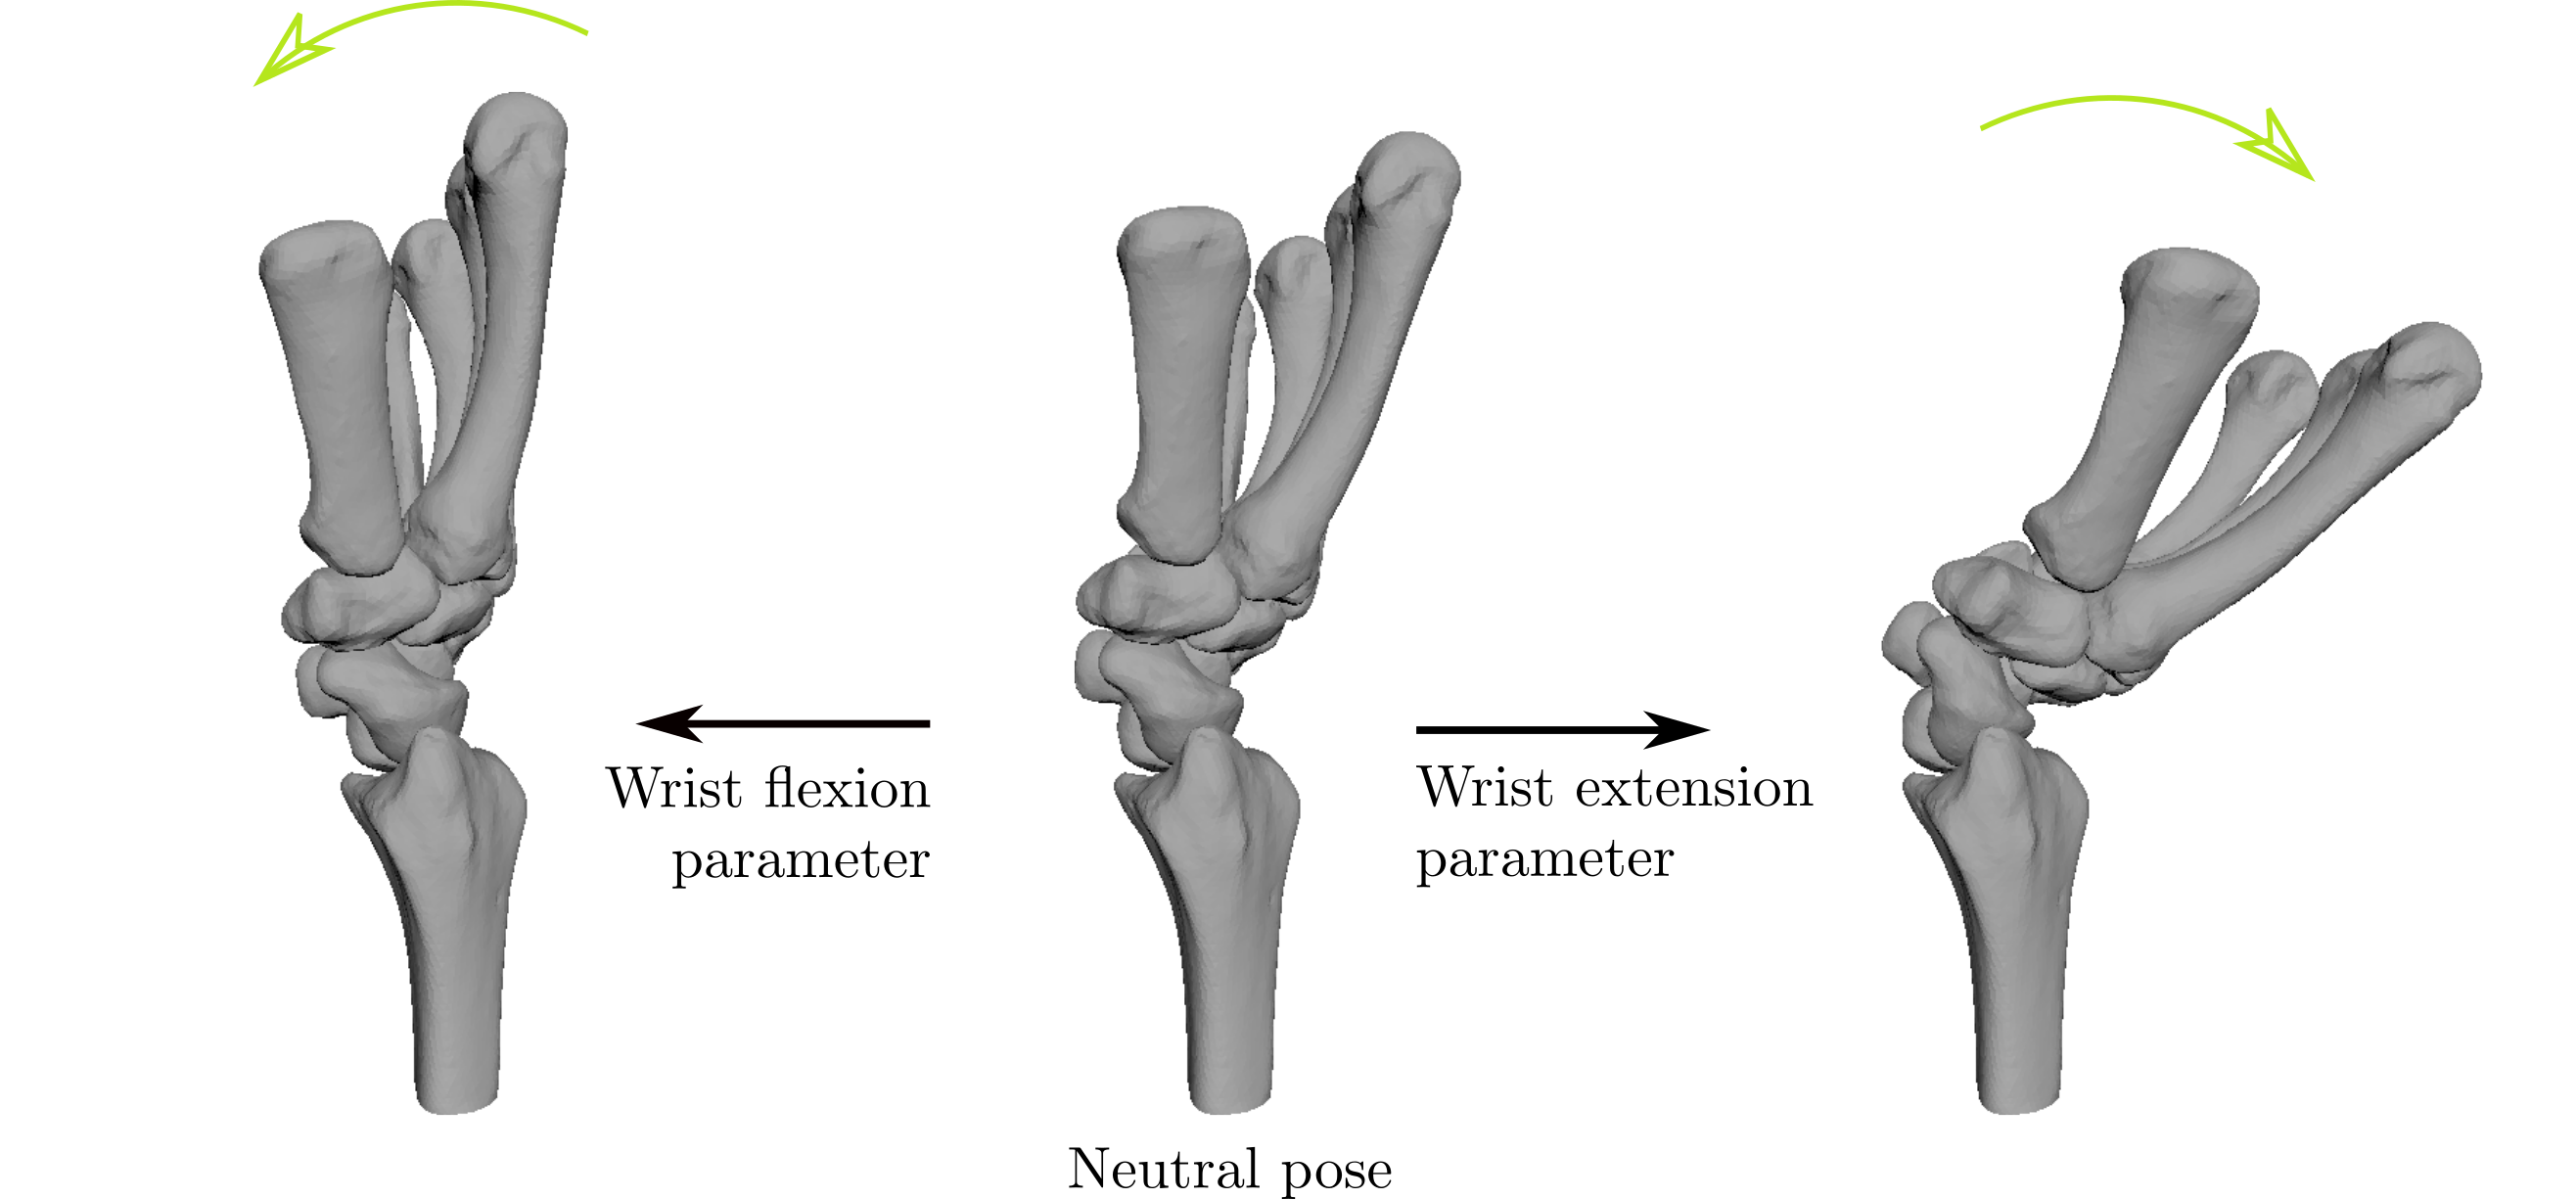
\includegraphics[width=0.95\textwidth]{\RootDir{img/wrist_flexext.png}}
	\caption{Wrist pose variations simulated by the model for the two extreme values of the wrist \fe* parameter}
	\label{im:5_wrist_flexext}
\end{figure}


\begin{figure}
	\centering
	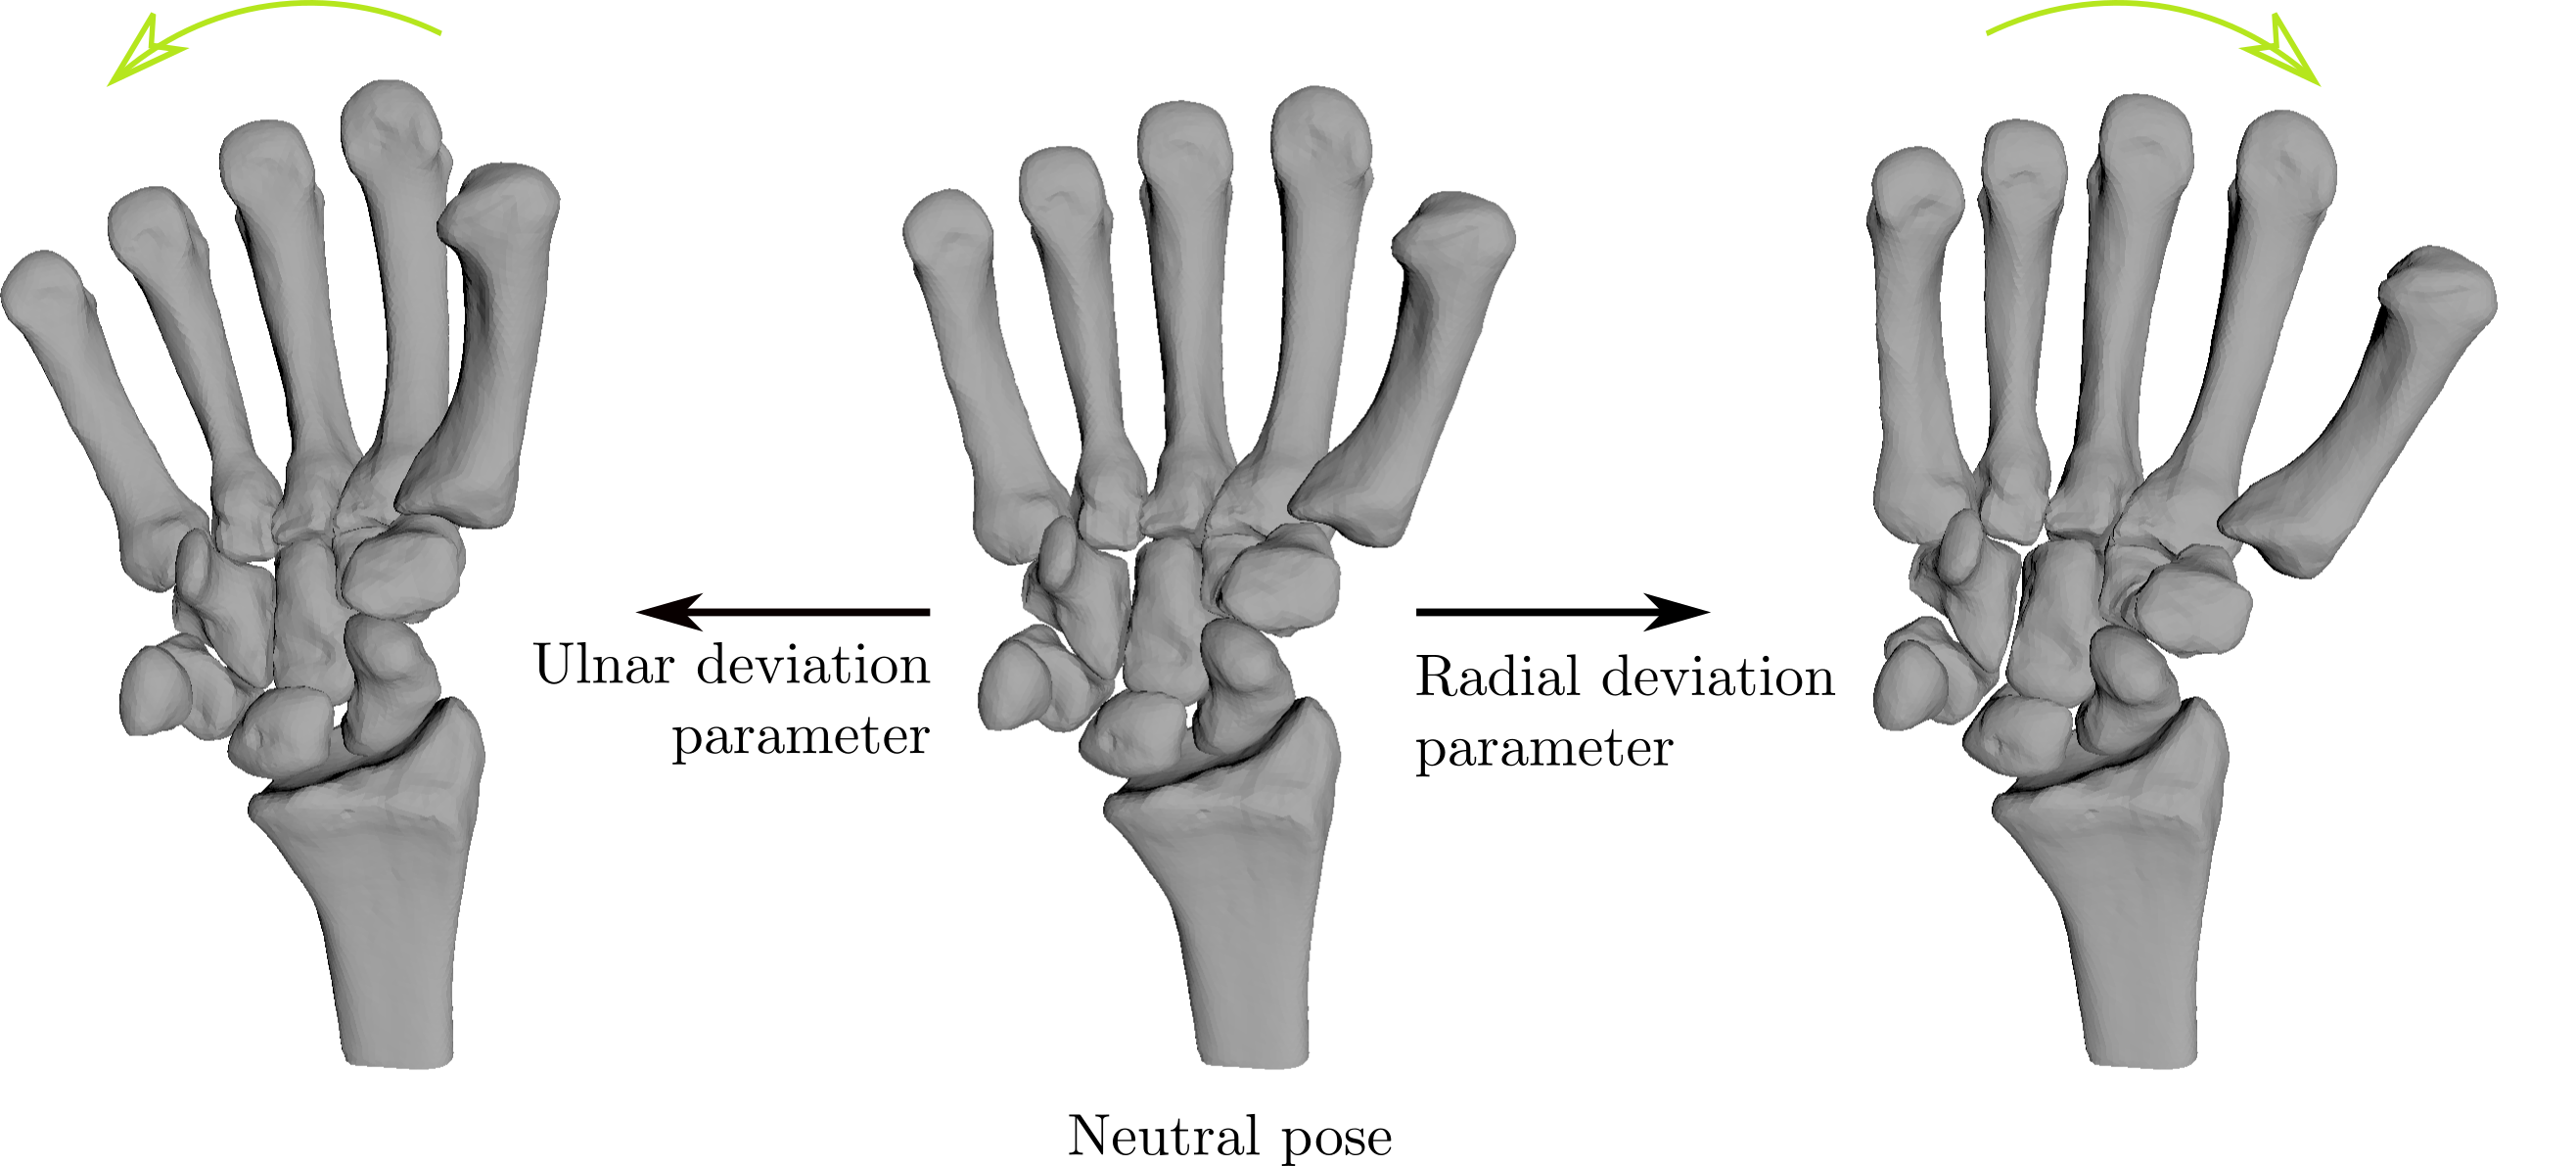
\includegraphics[width=0.9\textwidth]{\RootDir{img/wrist_dev.png}}
	\caption{Wrist pose variations simulated by the model for the two extreme values of the wrist deviation parameter}
	\label{im:5_wrist_deviation}
\end{figure}


\begin{figure}
	\centering
	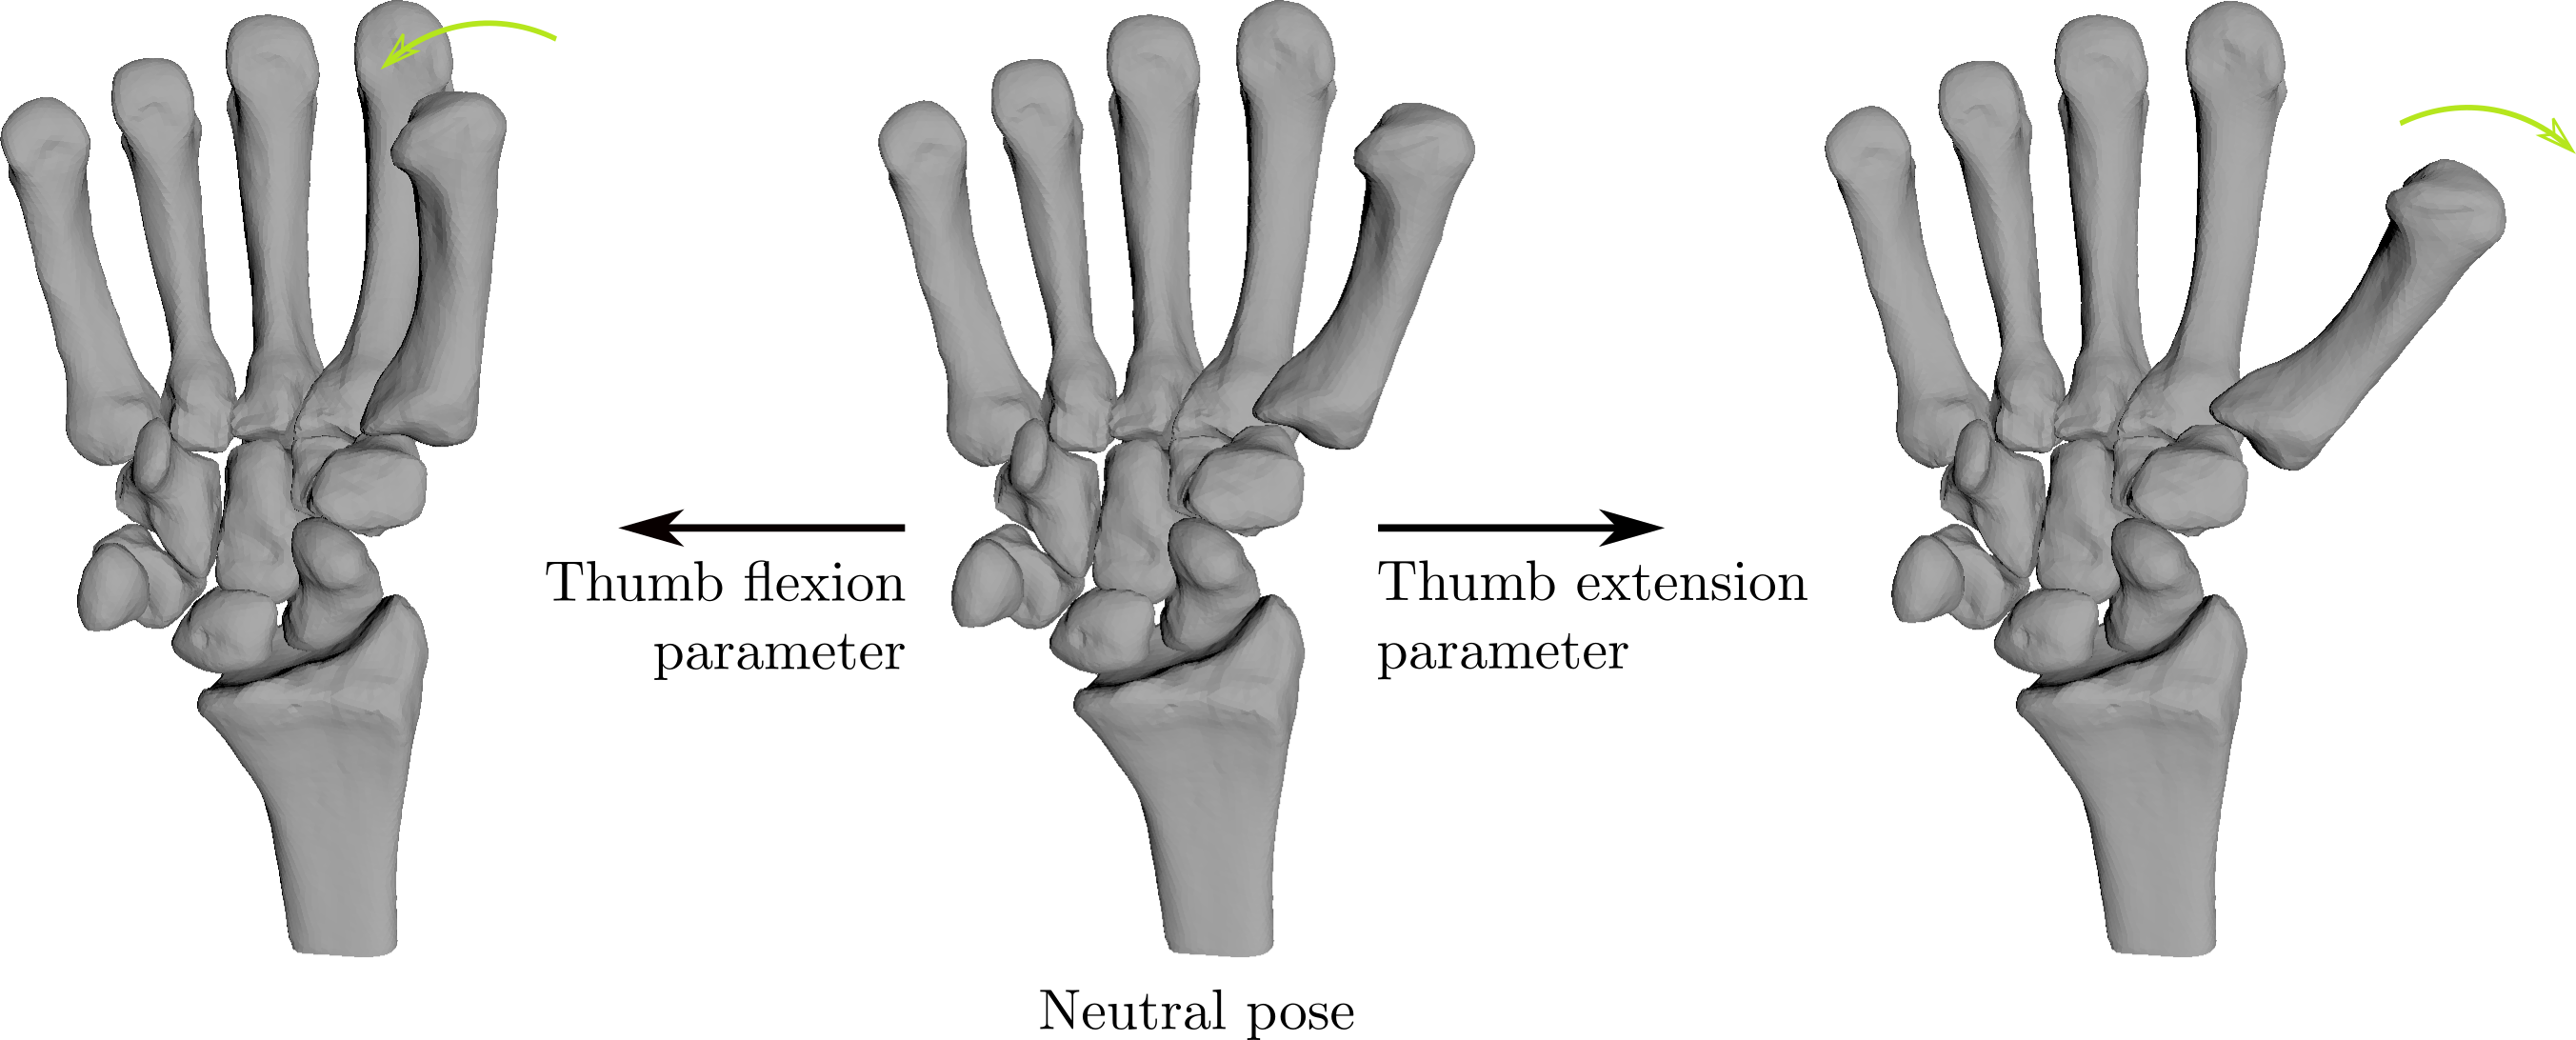
\includegraphics[width=0.9\textwidth]{\RootDir{img/thumb_flexext.png}}
	\caption{Wrist pose variations simulated by the model for the two extreme values of the thumb \fe* parameter}
	\label{im:5_thumb_fe}
\end{figure}


\begin{figure}
	\centering
	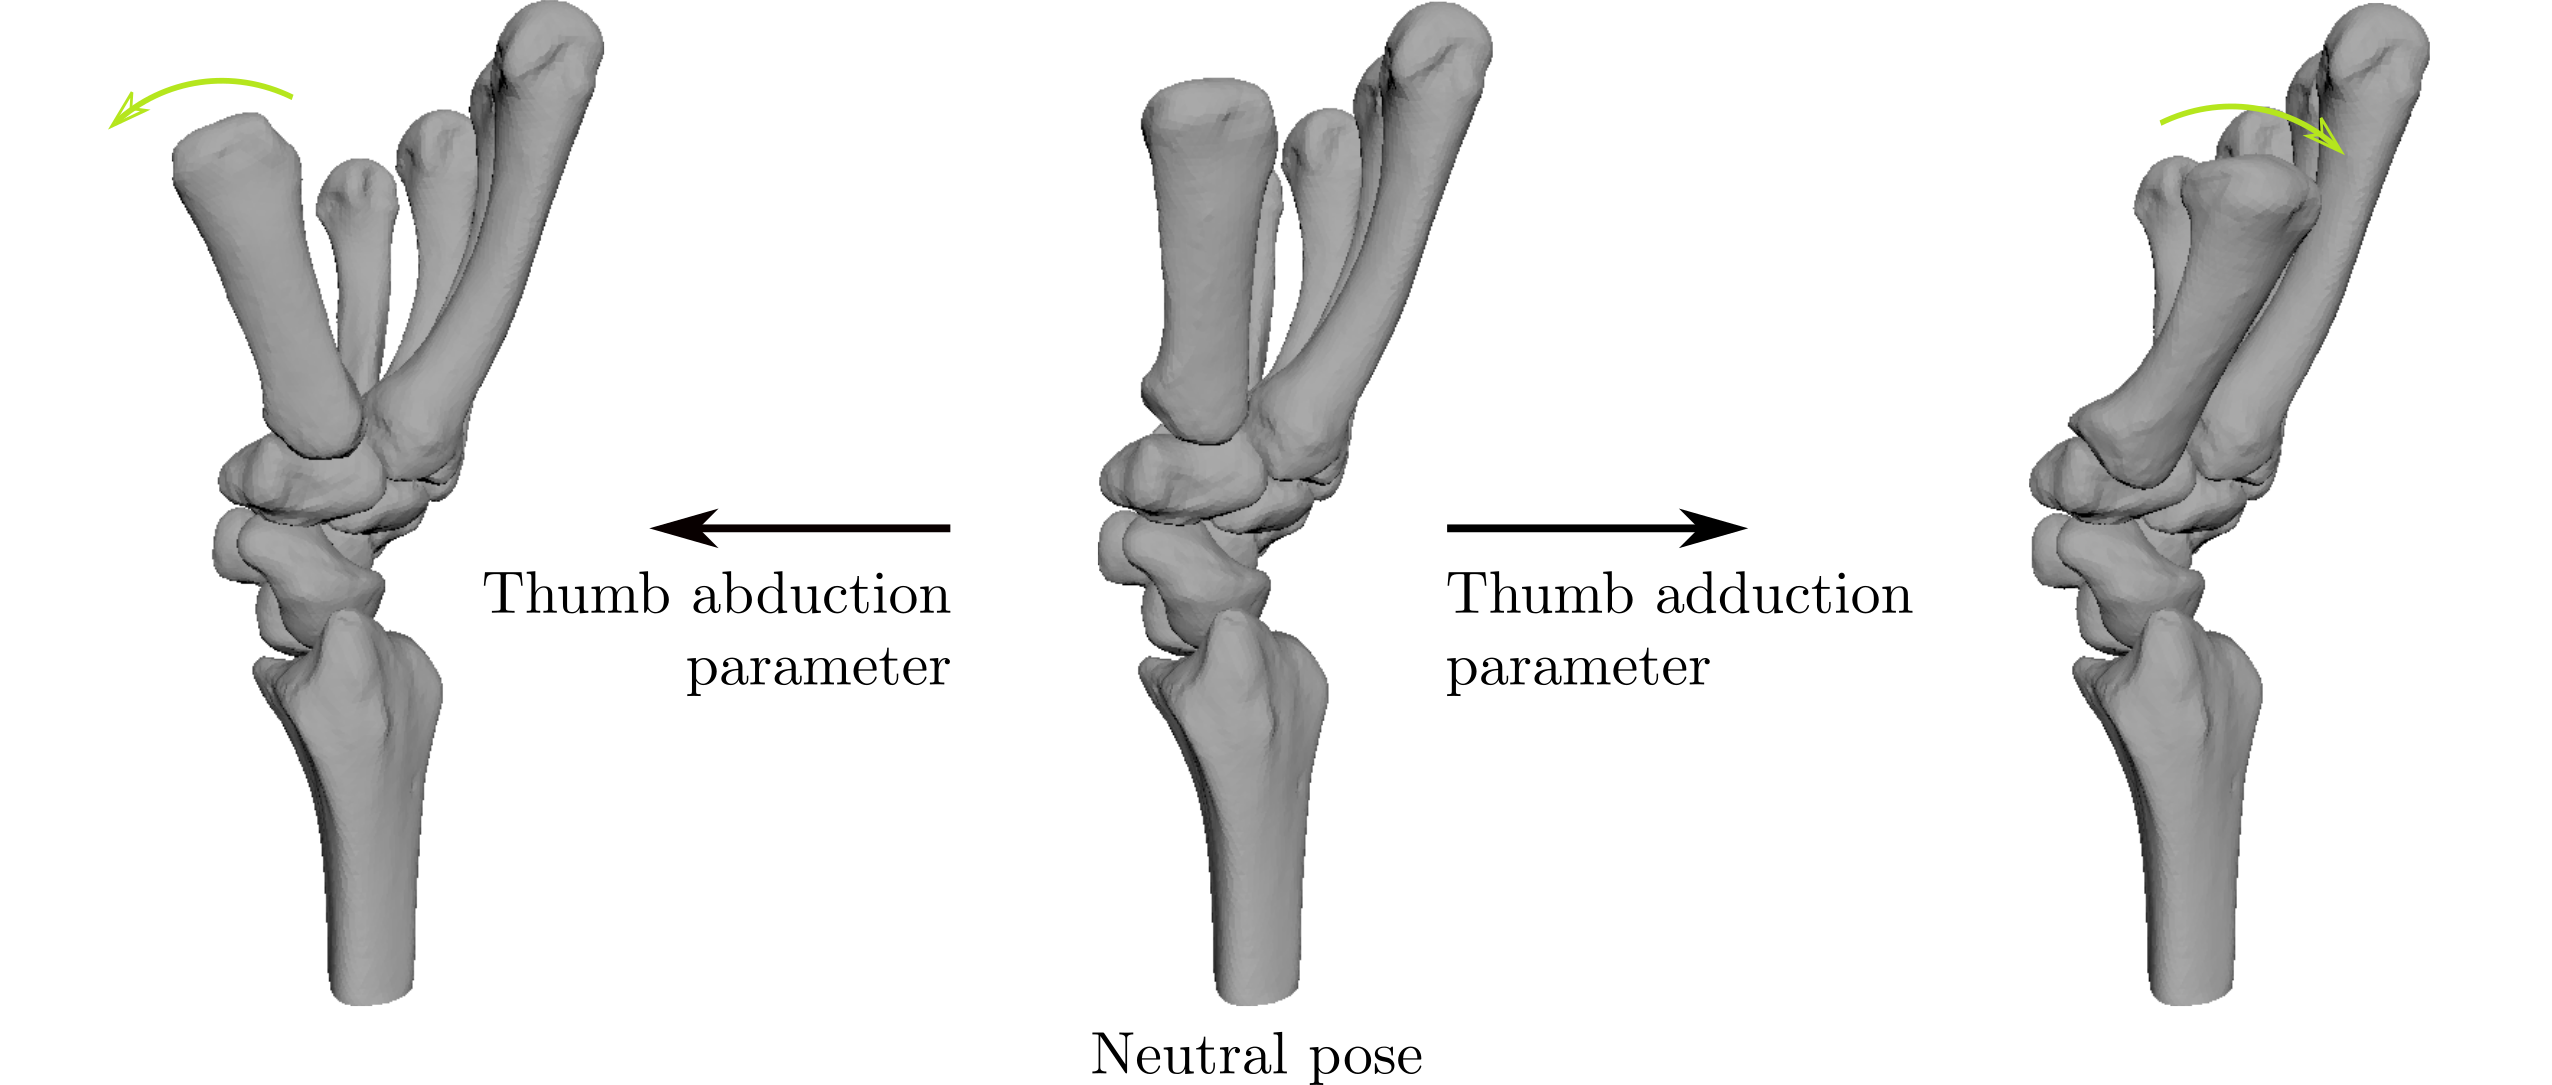
\includegraphics[width=0.9\textwidth]{\RootDir{img/thumb_abdadd.png}}
	\caption{Wrist pose variations simulated by the model for the two extreme values of the thumb \aa* parameter}
	\label{im:5_thumb_aa}
\end{figure}


\begin{figure}[!ht]
	\centering
	\begin{subfigure}[b]{0.45\textwidth}
		\centering
		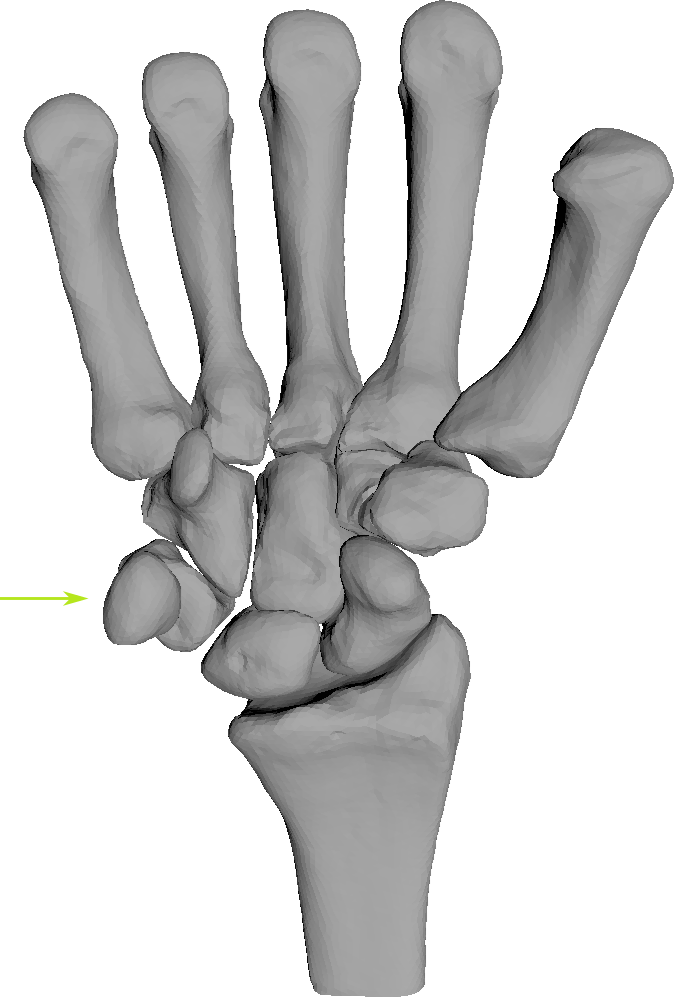
\includegraphics[width=0.6\textwidth]{\RootDir{img/unloaded.png}}
		\caption{Unloaded}
	\end{subfigure}
	~
	\begin{subfigure}[b]{0.45\textwidth}
		\centering
		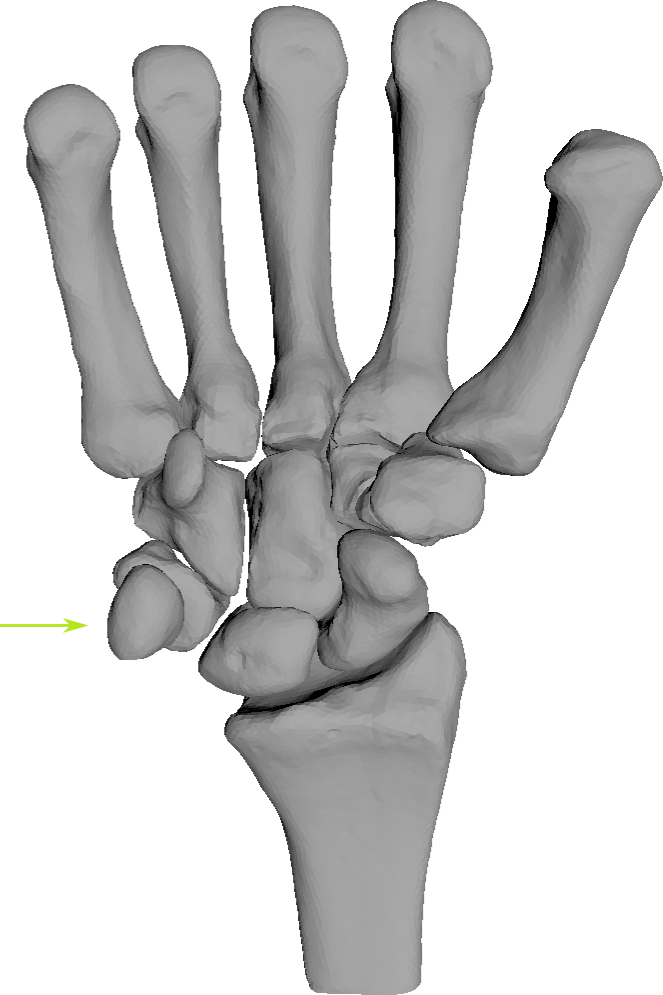
\includegraphics[width=0.6\textwidth]{\RootDir{img/loaded.png}}
		\caption{Loaded}
	\end{subfigure}
	
	\caption{Wrist pose variations simulated by the model for the boolean \textit{loaded} parameter}
	\label{im:5_loaded_param}
\end{figure}


It can be observed in the figures that the model has globally the expected behaviour: the correct wrist or thumb movement is performed. %The parameters seem to be adequate. 
In \figref{im:5_loaded_param} the effects of the force parameter are difficult to observe: the carpal bones are slightly drawn closer from each other, on the images only the pisiform displacement is visible, pointed out by arrows. It can also be noted that in \figref{im:5_wrist_flexext} the wrist flexion is barely visible. This is due to the absence of wrist flexion in the database poses. We observe a slight correlation between the wrists movements and the thumb ones: when the wrist is moved the thumb undergoes a light shift and the same happens in the other way around. It is hardly observable on the 2D pictures, for it is a very small fluctuation. The wrist and the finger movements are not completely decorrelated: it is the tenodesis effect. Due to the attachment of the finger tendons to the bones, the wrist joint movement influences the finger position \cite{revol_2010_tenodeses}. It can be observed for example when the wrist is flexed, if the fingers are free they have a tendency to stretch out, while they bend with an extension movement. The correlation observed in the model must be further analyzed with additional data to check if it is completely due to the tenodesis effect, or if a part of it originates from the poses learned in the training set, which present no wrist only motion.


Different types of representation of the data were tested: in the example model in \figref{im:5_wrist_flexext} to \figref{im:5_loaded_param} each bone was considered independently of the others. Using hierarchy between the bones was also tried out: the movement of a bone is expressed relatively to the previous one in the chain of articulation. \mcu* is dependent on \tpm*, \mcd* depends on the trapezoid, \mct* is related to \capitate* and finally \mcq* and \mcc* are linked to \ham*. The carpal bones relationships are too complex, we didn't try to create a hierarchy between them. This data representation didn't have much impact on the model and the parameters effects. Different functions $\Phi_j$ were also tested including radial basis functions and various values for the regularization parameter $\lambda$. We introduce two example models that were used to test the generalization capacity of the model. 

\paragraph{Model 1}
\label{model1}
\begin{itemize}
	\item $\Phi_j(x_j) = x_j$; 
	\item  $\lambda = 0;$ 
	\item No hierarchy between the bones
\end{itemize}

\paragraph{Model 2}
\label{model2}
\begin{itemize}
	\item $\Phi_j(x) = \exp\left(-\frac{1}{2} \frac{\norm{x_j - \bar{x_j}}^2}{\sigma^2} \right)$; $\bar{x_j}$ is the mean value of the $j^{th}$ predictor over all training observations
	\item $\sigma = 24.0$  
	\item  $\lambda = 0.05;$
	\item No hierarchy between the bones
\end{itemize}

The generalization capacity of the model was tested with the two parameterizations presented above. By turn one pose was left out of the training set of all poses for one individual, and using the predictor values, positions and orientations of the bones for the pose were calculated with the model. The values are compared to the experimental values obtained from the poses scans. The average position and orientation errors over all individuals are computed, the bones are considered separately. The difference of orientation is given as a global angle, the angle of rotation around the helical axis describing the motion to go from the computed orientation to the experimental one. The position error is given as a global distance in mm. We present the errors made with Model \hyperref[model1]{1} and Model \hyperref[model2]{2} for 4 bones: for \mcu* in \tabref{tab:linreg_mc1}, for \mct* in \tabref{tab:linreg_mc3}, for \lun* in \tabref{tab:linreg_lun} and finally for \ham* in \tabref{tab:linreg_ham}. An example of an experimental and the equivalent calculated pose is presented in \figref{im:5_generalization_pose}: the experimental bone positions and orientations are in orange, while the gray bones were calculated with Model \hyperref[model1]{1} in the "Jar, no load" pose.

\begin{table}[!ht]
	\centering
	\begin{tabular}{lcc|cc}
		\toprule
			\mcu* & \multicolumn{2}{c}{Model \hyperref[model1]{1}} & \multicolumn{2}{c}{Model \hyperref[model2]{2}} \\
			Pose & Translation (mm) & Rotation (\degre) & Translation (mm) & Rotation (\degre) \\
		\midrule
			Neutral 		 & 1.104 	 & 1.547 	 & 1.151 	 & 4.800 \\
			Adduction 		 & 0.989 	 & 0.983 	 & 1.709 	 & 2.294 \\
			Abduction 		 & 0.945 	 & 0.296 	 & 1.652 	 & 1.637 \\
			Extension 		 & 0.884 	 & 0.822 	 & 1.519 	 & 1.886 \\
			Flexion 		 & 0.840 	 & 1.098 	 & 1.780 	 & 1.349 \\
			Pinch, no load 	 & 0.851 	 & 1.132 	 & 1.609 	 & 1.189 \\
			Pinch, loaded 	 & 0.808 	 & 0.837 	 & 1.514 	 & 1.148 \\
			Grasp, no load 	 & 0.804 	 & 0.734 	 & 1.448 	 & 1.012 \\
			Grasp, load 	 & 0.770 	 & 0.702 	 & 1.391 	 & 0.547 \\
			Jar, no load 	 & 0.745 	 & 0.682 	 & 1.350 	 & 0.413 \\
			Jar, load 		 & 0.731 	 & 0.526 	 & 1.372 	 & 0.126 \\
		\bottomrule
	\end{tabular}
	\caption[Generalization capacity of the statistical movement model for the \mcu*]{Average error over individuals between the experimental orientation and position of the \mcu* and the values computed from the predictors, using two linear regression sets of parameters.}
	\label{tab:linreg_mc1}
\end{table}



\begin{figure}
	\centering
	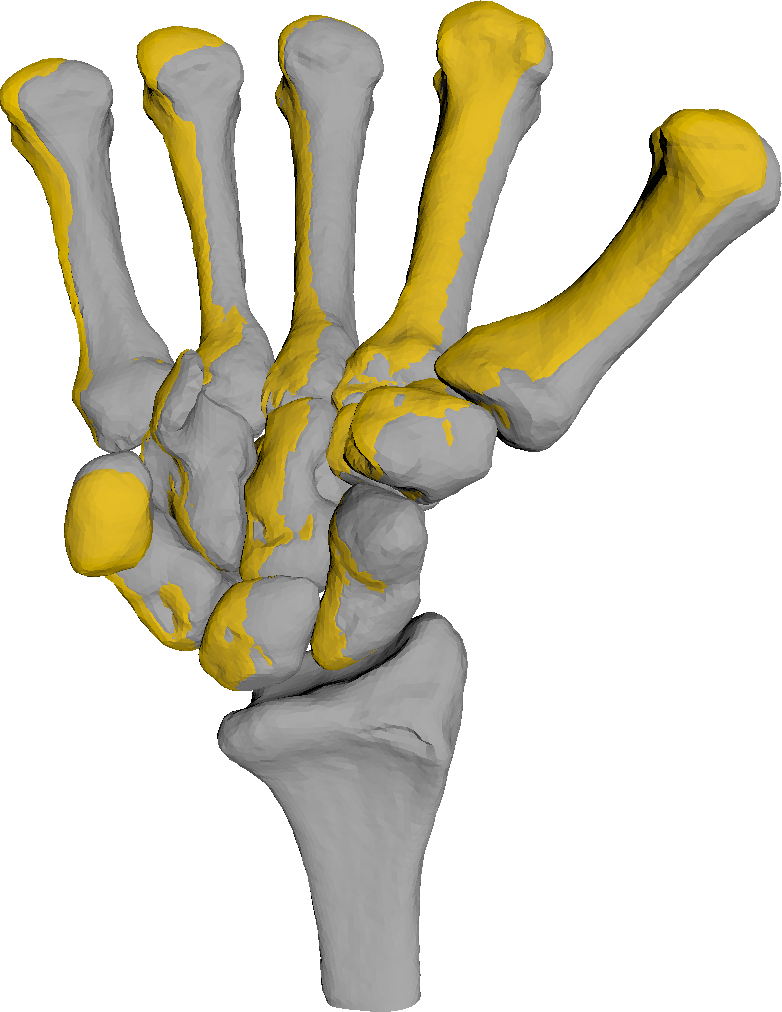
\includegraphics[width=0.5\textwidth]{\RootDir{img/jar_no_load_linreg_simple.png}}
	\caption[Computation of a pose with the movement model from the predictor values]{Simulation of the "Jar, no load" pose with the Model \hyperref[model1]{1}, while the pose was left out of the training set. In orange are the experimental bones as captured in the database, in gray the positions and orientations of the bones computed with a linear regression model, using the predictors values. }
	\label{im:5_generalization_pose}
\end{figure}


In Tables \ref{tab:linreg_mc1}, \ref{tab:linreg_mc3}, \ref{tab:linreg_lun}, \ref{tab:linreg_ham} are presented the average differences in location and orientation between the experimental poses and the ones calculated with linear regression for two sets of parameters for 4 bones: \mcu*, \mct*, \lun* and \ham*. These values are hardly interpretable in themselves. In Tables \ref{tab:5_average_transfo_to_poses_mcu_mct} and \ref{tab:5_average_transfo_to_poses_lun_ham} are given as indications the mean translation and rotation values of the same bones between the neutral pose and all other poses. The errors must be compared relatively to the ranges of rotation and translations the bones undergo during motion.


\begin{table}[!ht]
	\centering
	\begin{tabular}{lcc|cc}
		\toprule
		& \multicolumn{2}{c}{\mcu*} & \multicolumn{2}{c}{\mct*}  \\
		Pose & Translation (mm) & Rotation (\degre) & Translation (mm) & Rotation (\degre) \\
		\midrule
		Thumb Adduction & 3.18 & 9.73 & 0.64 & 2.23 \\
		Thumb Abduction & 2.84 & 13.45 & 0.60 & 5.24 \\
		Thumb Extension & 3.52 & 29.38 & 0.73 & 5.78 \\
		Thumb Flexion & 3.19 & 10.78 & 0.66 & 5.38 \\
		Pinch, no load & 2.54 & 20.61 & 0.79 & 7.95 \\
		Pinch, loaded & 2.15 & 16.54 & 1.03 & 12.00 \\
		Grasp, no load & 3.90 & 21.98 & 1.46 & 27.60 \\
		Grasp, load & 6.59 & 40.11 & 1.37 & 37.60 \\
		Jar, no load & 5.97 & 31.42 & 1.81 & 33.73 \\
		Jar, load & 3.40 & 13.33 & 1.67 & 22.00 \\
		\bottomrule
	\end{tabular}
	\caption[Average transformation from neutral pose to all other for the \mcu* and \mct*]{Average rotation and translation in absolute values over individuals between the neutral pose and the other experimental poses for the \mcu* and \mct* bones in the \db*.}
	\label{tab:5_average_transfo_to_poses_mcu_mct}
\end{table}

It must be noted that there are few training poses and leaving one out to test the model necessarily skew the results. Some extreme poses such as the thumb flexion and extension ones should be used to define the space of possible poses. However there are not enough poses to both test the generalization capacity and leave all extreme poses out of the test procedure. 


